\documentclass[UTF8]{ctexart}
\usepackage{bookmark}
\usepackage{hyperref}
\usepackage{geometry}
\geometry{a4paper,scale=0.8}
\usepackage{ctex}
\usepackage[style=caspervector,backend=biber,utf8]{biblatex}
\addbibresource{reference.bib}
\usepackage{booktabs}
\usepackage{array}
\usepackage{fancyhdr}
\pagestyle{fancy}
\fancyhf{}
\renewcommand\footrulewidth{1pt}
\lhead{王铠泽}
\rhead{PB18020766}
\chead{\href{mailto:volar@mail.ustc.edu.cn}{volar@mail.ustc.edu.cn}}
\rfoot{中国科学技术大学}
\lfoot{\today}
\usepackage{graphicx}
\usepackage{float}
\usepackage{subfigure}


\begin{document}

	\centering\textbf{\LARGE{计算物理A第四次作业}}
	
	
	王铠泽\qquad PB18020766
	
		
	\section{作业题目}
	
	\begin{itemize}
		\item 设概率密度函数满足关系式:
		$$p(x)=\frac{dp(x)}{dx}\frac{x-d}{ax^2+bx+c}$$
		请找到其中的一种函数,讨论其性质,并给出抽样方法。
		
		\item
		尝试两个不同组合$(a,b,c,d)=(1,1,1,1)/(-1,1,1,1)$,得到一般的图像大概如下:
		
		\begin{figure}[H]
			\centering  %图片全局居中
			\subfigure[$(a,b,c,d)=(1,1,1,1)$]{
				
				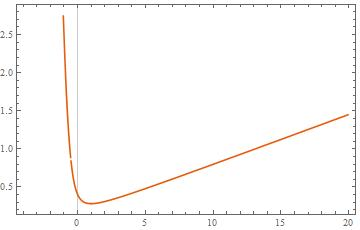
\includegraphics[width=0.4\textwidth]{../4.jpg}}
			\subfigure[$(a,b,c,d)=(-1,1,1,1)$]{
				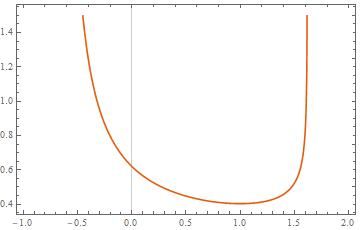
\includegraphics[width=0.4\textwidth]{../3.jpg}}
			
			\caption{函数形态}
			\label{N}
		\end{figure}
		
	\end{itemize}
	
	\section{实现方法}
	\begin{flushleft}
		本实验着重讨论两种情况,分别提取出分母平方项和一次方项的特征,令$$(a,b,c,d)=(-1,0,1,0),(a,b,c,d)=(0,-2,1,0)$$
	即:
	\end{flushleft}
	$$p_1(x)=\frac{1}{\pi}\frac{1}{\sqrt{1-x^2}}\cdot I(-1\leq x\leq 1)$$
	$$p_2(x)=\frac{1}{A}\frac{e^{-x}}{{(x-2)}^2}\cdot I(-1\leq x\leq1)$$
\begin{flushleft}
		其中$I(-1\leq x\leq1)$为示性函数,表示对$x$取值的限制。其取值为:
\end{flushleft}
	$$I(-1\leq x\leq1)=\left\{
	\begin{array}{lr}
	1&-1\leq x\leq 1\\
	0& otherwise
	\end{array}
	\right.$$
	后面将自动略去示性函数,默认$p(x)$定义在$[-1,1]$上。
	\begin{flushleft}
		使用$Mathematica$的数值积分功能得到$A=0.549707$,$\frac{1}{A}\approx1.81915$。
	
		函数图像如下:
	\end{flushleft}
	
	\begin{figure}[H]
				\centering  %图片全局居中
				\subfigure[{$\frac{1}{\pi}\frac{1}{\sqrt{1-x^2}}$}]{
					
					\includegraphics[width=0.4\textwidth]{../1.jpg}}
				\subfigure[$\frac{1}{A}\frac{e^{-x}}{{(x-2)}^2}$]{
					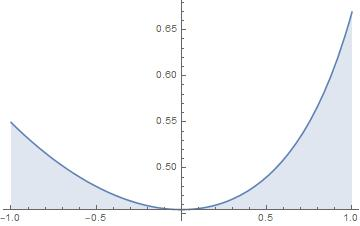
\includegraphics[width=0.4\textwidth]{../2.jpg}}
				
				\caption{$p_1(x),p_2(x)$函数图像}
				\label{N}
	\end{figure}
		在本次实验中,采用的是16807产生器(最低标准产生器),即 $a=16807,b=0,m=2^{31}-1$。
	\begin{itemize}
		
		\item 直接抽样法
		
		对于$p_1(x)=\frac{1}{\pi}\frac{1}{\sqrt{1-x^2}}$采用简单抽样。先求累计函数$F(x)$:
		$$F(x)=\int_{-1}^{x}p_1(\xi)d\xi=\frac{1}{\pi}arcsin(x)+\frac12$$
		
		采用16807产生器生成随机序列$\xi$,则目标抽样为
		$$x=sin[\pi(\xi-\frac{1}{2})]$$
		这和$x=sin(2\pi\xi)$的抽样等价。
		
		\item 舍选抽样法
		
		由于对于$p_2(x)=\frac{1}{A}\frac{e^{-x}}{{(x-2)}^2}$没有解析的累计函数,另一方面若想采用变换抽样法比较难以找到合适的变换使得$|J|=p_2(x)$。所以只能舍弃一些效率选用舍选抽样法。
		
		采用$F(x)=\frac{1}{\sqrt{3-x^2}}$作为覆盖$p_2(x)$的比较函数。$I=\int_{-1}^{1}F(x)dx=2sin^{-1}(\frac{1}{\sqrt{3}})$。该舍选效率为:
		$$Area[p_2(x)]/Area[F(x)]\approx0.812374$$
		
			\begin{figure}[H]
			\centering  %图片全局居中
			
				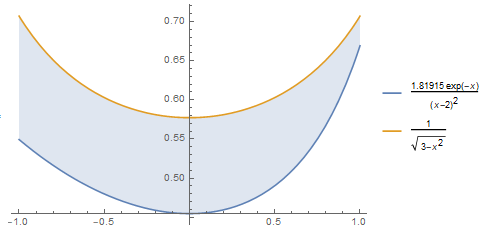
\includegraphics[width=4in]{F.png}
			\caption{$F(x),p_2(x)$函数图像}
			\label{N}
		\end{figure}
	抽样方法:
	生成两个$[0,1]$上随机序列$\xi_1
	,\xi_2$。在$x$方向上,按$F(x)$分布抽样:$$\xi_x=\sqrt{3}sin[2sin^{-1}(\frac{1}{\sqrt{3}})(\xi_1-\frac{1}{2 })]$$
	在$y$方向上,按$\frac{1}{F(\xi_x)}$的均匀分布抽样:$$\xi_y=F(\xi_x)\xi_2$$
	比较关系:
		$$\left\{
		\begin{array}{lc}
		\xi_y<p_2(\xi_x)& accept\\
		\xi_y\geq p_2(\xi_x)& reject\\
		\end{array}
		\right.
		$$
	\end{itemize}
	\section{程式说明}
	
	\begin{itemize}
		\item rdm.h
		
		这是一个包含了使用16807产生器生成指定长度的$[0,1]$上均匀分布随机数函数的头文件。
		
		\subitem void rdm(int N,double *x,int method)
		
		该函数将输入的指针$x$对应的长度为$N$的数组用$[0,1]$上的随机数填满。method是关于初始种子的选择。method=0:默认种子;method=1,时间种子。
		
		本次实验中,在生成$\xi_1,\xi_2$时,为了保证独立性,分别采用默认种子和时间种子。
		\item pdf\_sampling\_1.c 
		
		该程式产生按$p_1(x)$分布进行抽样的一组指定个数($N$)的随机数。	
		
		\item pdf\_sampling\_2.c
		
		该程式产生按$p_2(x)$分布进行抽样的一组指定个数($N$)的随机数。
		
		\item time\_seed.txt
		
		该文本文件显示的是调用时间种子时对应的原始数据。
		
		\item p\_1(x).txt p\_2(x).txt
		
		分别记录根据$p_1(x),p_2(x)$为密度函数生成的随机序列。
	\end{itemize}
	
	\section{计算结果}

		下面根据数据使用$ Python $程序做出频数分布直方图,检验生成随机序列。
			预设$bin=500$,$p_1(x)$总点数$N=10000$;$p_2(x)$未舍选之前总点数为$N=10000$,$N=100000,N=1000000$。
			
			实际效率为:0.809300,0.811870,0.812796。


%	\begin{figure}[H]
%	\centering\includegraphics[width=2in]{1.jpg}
%	\caption{something}\label{fig:1}
%	\end{figure}
	\subsection{直方图检验}
	\begin{figure}[htbp]
		\centering  %图片全局居中
		\subfigure[$p_1(x)$序列,$N=10000$]{
	
			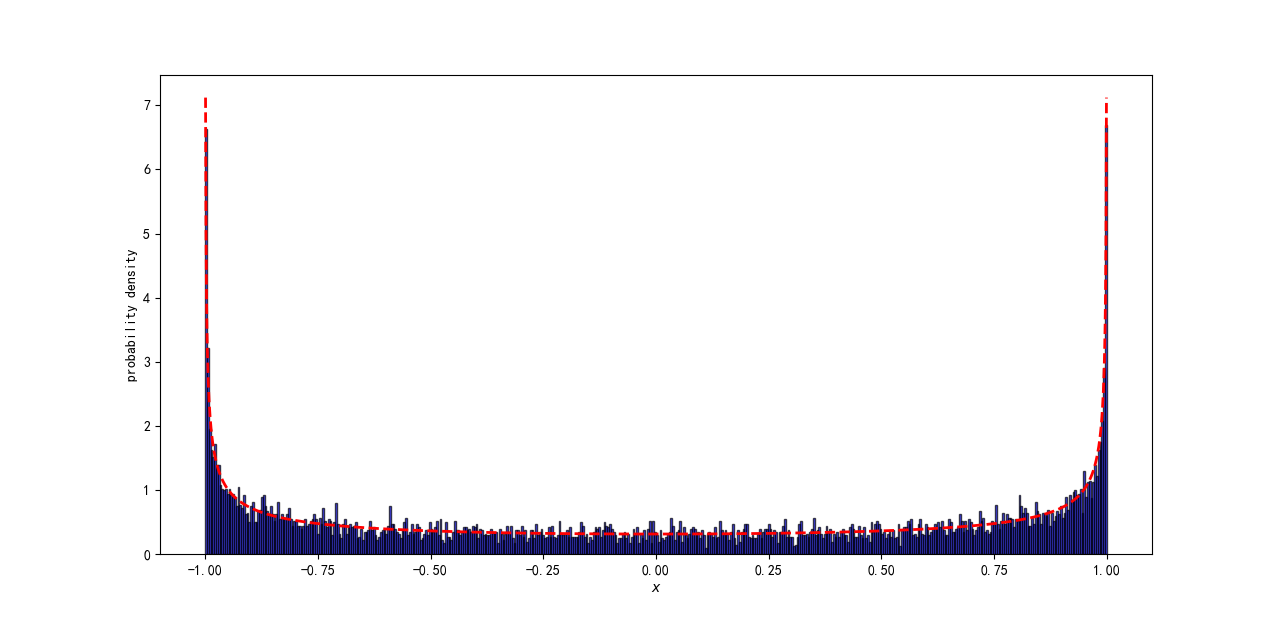
\includegraphics[width=0.6\textwidth]{../p_1.png}}
			\subfigure[$p_2(x)$序列,$N=10000$]{
			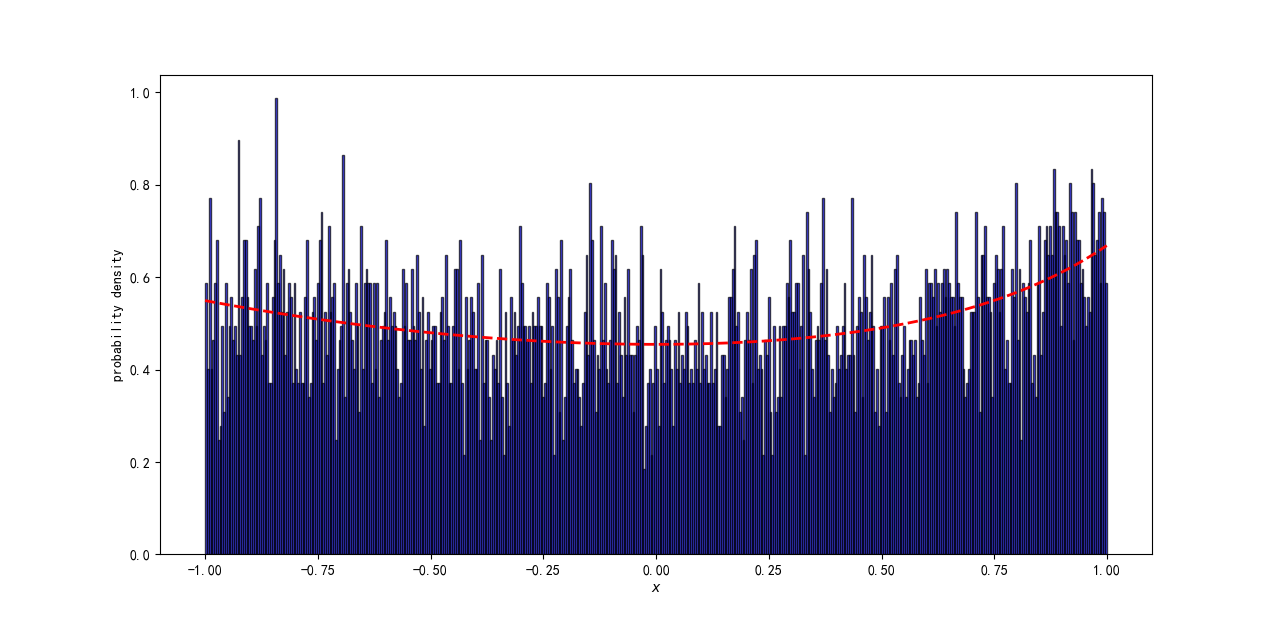
\includegraphics[width=0.6\textwidth]{../p_20.png}}
		\subfigure[$p_2(x)$序列,$N=10000$]{
			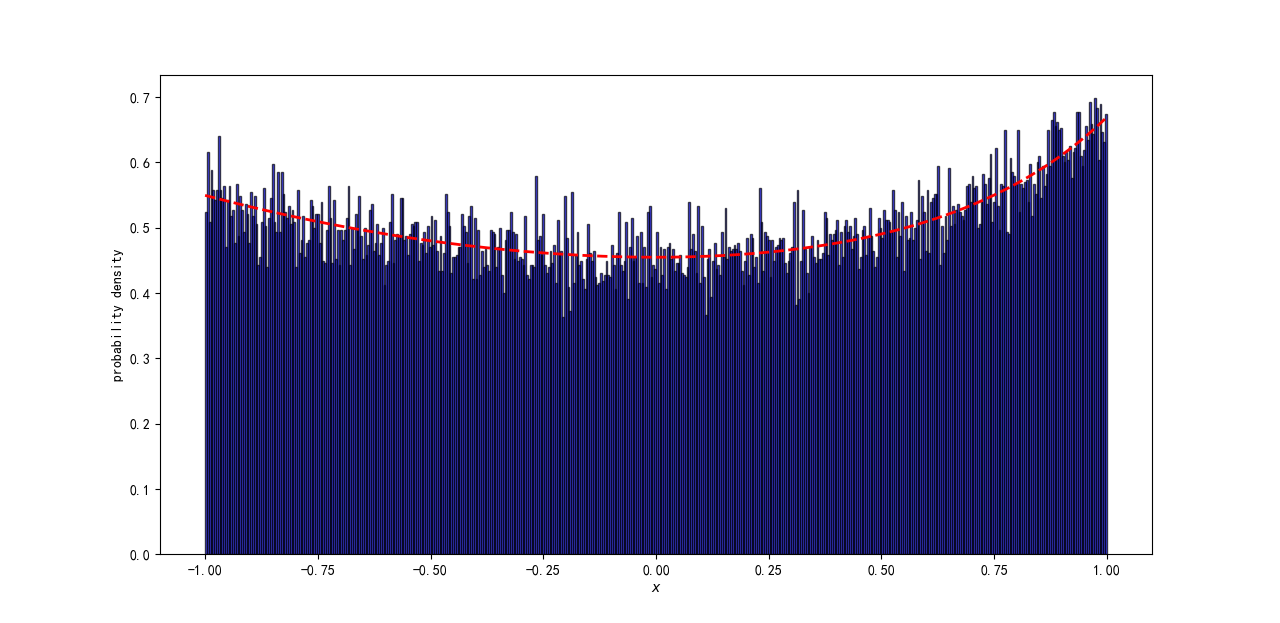
\includegraphics[width=0.6\textwidth]{../p_2.png}}
		\subfigure[$p_2(x)$序列,$ N =1000000$]{
			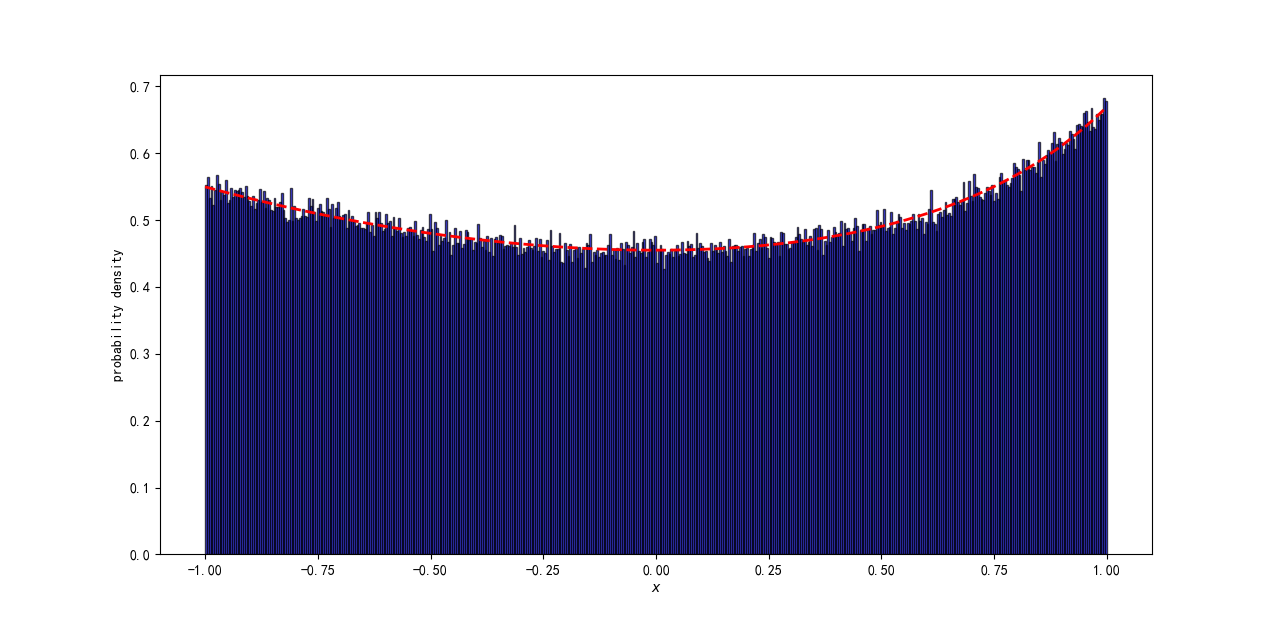
\includegraphics[width=0.6\textwidth]{../p_22.png}}
		\caption{直方图检验(红色虚线为理想分布)}
		\label{N}
	\end{figure}
	
	\begin{flushleft}
		可见,$p_1(x)$序列采用直接抽样法,在点数较少的情况下收敛情况良好。而$p_2(x)$序列由于采用的是舍选法,需要更多的点数来得到良好收敛的概率密度函数。
	\end{flushleft}
	
	\section{总结}
	\begin{itemize}
		\item 当累计函数难以求得反函数时,舍选法是一个有效得到抽样的方法,但是其效率会降低,需要仔细地选择合适的比较函数。选择比较函数,一方面要尽可能和抽样函数形状,趋势一致,另一方面,还要容易求得反函数。本题中的比较函数$F(x)$其实和$p_1(x)$是同一类型函数,因而满足上述要求。
		
		\item 满足微分方程$p(x)=\frac{dp(x)}{dx}\frac{x-d}{ax^2+bx+c}$的函数往往在某点会发散,因而只能将其定义在某个区间上,甚至密度函数出现不连续点。
	\end{itemize}
	\clearpage
\end{document}